\chapter{Two TDP-43 mutant mice}

\section{Overview}
% work performed by myself, Dr Kitty Lo and Prasanth Sivakumar. Kitty Lo began the analysis and I finished it. Prasanth contributed the iCLIP and the wet lab validations

This chapter has been published as \citep{Fratta2018}
RT-PCR were performed, quantified and plotted by Prasanth Sivakumar.
RNA-seq and iCLIP libraries were created by Prasanth Sivakumar and Dr Agnieszka Gromadzka.
Mice were handled by ??? and Dr Cristian Bodo.
Preliminary analysis of splicing was performed by Dr Warren Emmett and Dr Kitty Lo.





\section{Background}




\section{Methods}
% drop in from paper as I wrote them

\subsection{Differential expression}
To assess the relationship between intron length and differential expression, I found the longest intron in each gene using annotations from GENCODE mouse release 25 \citep{Harrow2012} by writing a custom Python script (2.7.1). I converted unadjusted p-values from DESeq2 into Z-scores and given the sign of the $log_2$ fold change. Genes were ordered by signed Z-score and binned into groups of  200. The plots present the mean intron length and  standard error  of  the mean  for each group.  

I downloaded and processed RNA sequencing data from of TDP-43 knockdown in mouse adult striatum \citep{Polymenidou2011} using the same analysis pipeline and used as a positive control.


\subsection{Differential splicing}

Three different generations and qualities of sequencing data were generated over the course of the  study.  Therefore  the  methods I  used  to  measure  splicing  changes  were  tailored  to  each 
dataset. RNA sequencing allows for unambiguous assignment of splice events in the form of spliced junction reads. 
However, due to their rare occurrence compared to non junction-spanning reads, the number of junction reads detected in a sample and therefore the power to resolve differential splicing depends on the initial depth of sequencing, the length of sequencing reads and the expression level of the gene. Therefore for low depth sequencing data it is practical to instead infer splicing changes from quantifying read coverage across each exon and ignore junction information. This approach is exemplified by the DEXSeq package \citep{Anders2012} which we used to estimate splicing changes in the embryonic fibroblast and head samples.

When sequencing depth and read length is increased it is possible to more accurately measure splicing variation with spliced junction reads alone. The cassette exon is a splicing variant comprised of three spliced junction reads: two flanking junctions that connect the flanking exons to the central cassette exon and a single parent junction that excludes it. By taking the ratio of the inclusion junction counts over the total number of junctions we can estimate the percent spliced in (PSI) of the cassette exon \citep{Katz2010-ir}. By comparing samples across conditions we can estimate a $\Delta$PSI - the difference in PSI between cases and controls. A positive $\Delta$PSI indicates increased exon inclusion and negative $\Delta$PSI indicates increased exon skipping. 

Due the high depth and long read length of the RRM2mut embryonic brain and LCDmut adult spinal cord samples we used the SGSeq package \citep{Goldstein2016}. This creates a local splicing graph of connected spliced junction reads and determines the splicing events contained within. These events consist of cassette exons, retained introns, alternate $3'$ and $5'$ junctions, alternate first and last exons, and mutually exclusive exons and SGSeq allows for the possibility of multiple classes of splicing event to occur within  the same interval. SGSeq  then quantifies  the number of  reads in each sample  that support each splice event and these counts can be used with DEXSeq. 

I created Pie charts to show the proportions of different types of events in an analysis, breaking complex  events  down  and  counting  the  individual  events  separately.  For  the  remaining splicing analyses the cassette exon splicing events were focused upon.


\subsection{Permutation of splicing results}
I permuted the sample order of the 4 wildtype and 4 LCDmut homozygotes 50 times to get all possible permutations and reran the splicing analysis for each comparison. Distributions of P-values are presented as quantile-quantile plots to visualise the inflation from the expected distribution under the null hypothesis of there being no difference between the two groups. 

\subsection{Annotation of splicing events}
Due to the current interest in unannotated (novel or cryptic) splicing events, particularly those linked 
to TDP-43 depletion \citep{Humphrey2017, Ling2015}, there is a need for tools that identify and classify spliced junction reads that cannot be assigned to known transcripts. SGSeq has the option of incorporating  novel  junctions  into  its  splicing  graphs,  giving  equal  weight  to  novel  and  annotated splicing events. 
As transcript annotation progresses the number of novel splicing events will diminish over time, and for this reason we have chosen to define extreme splicing changes by the levels of inclusion rather 
than annotation, which will naturally include unannotated events. For cryptic exons we use percent 
spliced  in  (PSI)  in  our  control  samples  and  the   $\Delta$PSI  between  mutants  and  controls  to  select cassette exon splicing events that are barely included in controls ( $PSI_{control}$ < 5\%) and then more included in the mutants ( $\Delta$PSI > 5\%). What we call ``skiptic'' exons are extreme cassette exon skipping events, where an exon that is apparently constitutive ($PSI_{control}$ > 95\%) is then skipped in the mutants ($\Delta$PSI > 5\%).

\subsection{Motif analysis}
Exons were flanked by 100nt either side and FASTA sequence extracted. Motif discovery was run using the  MEME  motif  discovery  tool  \citep{Bailey2009-lw},  restricting  to  8  letter  motifs.  A  set  of  exonic sequences not found to be differentially spliced were used as a background. 

\subsection{Functional analysis of extreme cassette splice events}
Cassette exons and their parent introns were extracted from the SGSeq results.
A per-nucleotide list of  PhyloP  conservation  scores \citep{Pollard2010-fj} for  the mouse  aligned  to  59  other  vertebrates (mm10.60way.phyloP60way.bw) was downloaded from UCSC. Mean scores were calculated for each exon  using  bigWigSummary  (UCSC). The  extreme  cassette  exons  were  compared  to  all  exons annotated in the GENCODE mouse release 25. Cassette exon splicing can destabilise its host transcript with either its inclusion or exclusion leading to a downstream frameshift and the presence of premature termination codons (Lewis et al, 2003). 
To predict the functional consequences of exon inclusion or skipping on the host transcript a custom script was written in R that predicted the upstream and downstream exons that  flank the extreme cassette exons using both GENCODE annotation and the spliced reads in from the aligned RNA-seq samples. If both flanking exons were predicted to be in the coding sequence then the exon sequences were concatenated with and without the central exon and translated in silico in the predicted codon frame of the upstream exon. If skipping or inclusion of the central exon caused a frameshift and/or a premature stop codon this was noted. 
To  assess  the  correlation  between  the  presence  of  an  extreme  cassette  exon  and  changes  in expression of its host gene, the proportion of genes that are significantly up- or downregulated at FDR < 10\% was assessed in extreme cassette exons non-extreme cassette exons and as a control, genes with no cassette splicing expressed at a level at or greater than the most lowly expressed extreme exon gene. The proportions of up- and downregulated genes were compared between  the control genes and the two groups of cassette exon containing genes with a binomial test in R.   

\subsection{iCLIP analyses}
Analysis  of  high-throughput  iCLIP  libraries  was  conducted  using  the  iCount  pipeline,  mapping  reads  to  the mm10 build of the mouse geneome  Only  uniquely-mapped  sense  reads  from each dataset were used. All peak calling and false discovery rate correction was carried out as described in \citep{Huppertz2014-ip,Konig2010}. Replicates with similar pentamer enrichment profiles and read  counts were  grouped  for  subsequent analysis. Pentamer  counts and annotation  of  peaks  to genes were provided by iCount. Pentamer analyses were conducted on 30nt intervals immediately surrounding the crosslinked site. 
RNA maps were created  for groups of cassette exons by quantifying per-nucleotide iCLIP coverage across the entire length of each parent intron that contains the splice sites of each cassette exon. To maximise  potential  coverage,  I pooled together all  iCLIP  replicates created  by the Fratta lab with  TDP-43  iCLIP generated previously \citep{Rogelj2012}. Analysis was  then  restricted  to 300nt around  the parent intron splice sites and 300nt around the cassette exon splice sites. Per-nucleotide iCLIP coverage was defined as the number of overlaps with at least one iCLIP cluster at an individual nucleotide divided by the total number of exon sequences. Due to variance in exon lengths, it was simply noted whether the exon overlapped with at least one iCLIP cluster and this is plotted as a proportion of all exons with a separate axis. The 20 cassette exons with the greatest total coverage are plotted individually.

To assess  the  dependence between  iCLIP  coverage and  intron  length,  total TDP-43  iCLIP  coverage 
across  the entire length of genes was calculated and normalised  to give a per-nucleotide coverage 
proportion. Genes were divided into those contained introns >100kb (see above) and to whether they were  upregulated  or  downregulated in  the RRM2mut compared  to wildtype littermates.  Coverage distributions were compared using a Mann-Whitney-Wilcoxon non-parametric test in R.

\subsection{Statistical analyses}
All differential expression results are significant at a Benjamini-Hochberg false discovery rate of 10\%. 
All  differential  splicing  results  presented  are  significant  at  a  false  discovery  rate  of  1\%  unless specifically stated.



\section{Results}

\subsection{A random mutagenesis screen produces two mutant mouse lines with point mutations in \textit{Tardbp}}

% figure showing both mutations within the structure of TDP-43
\begin{figure}[h!]
	%\begin{center}
		\centering
		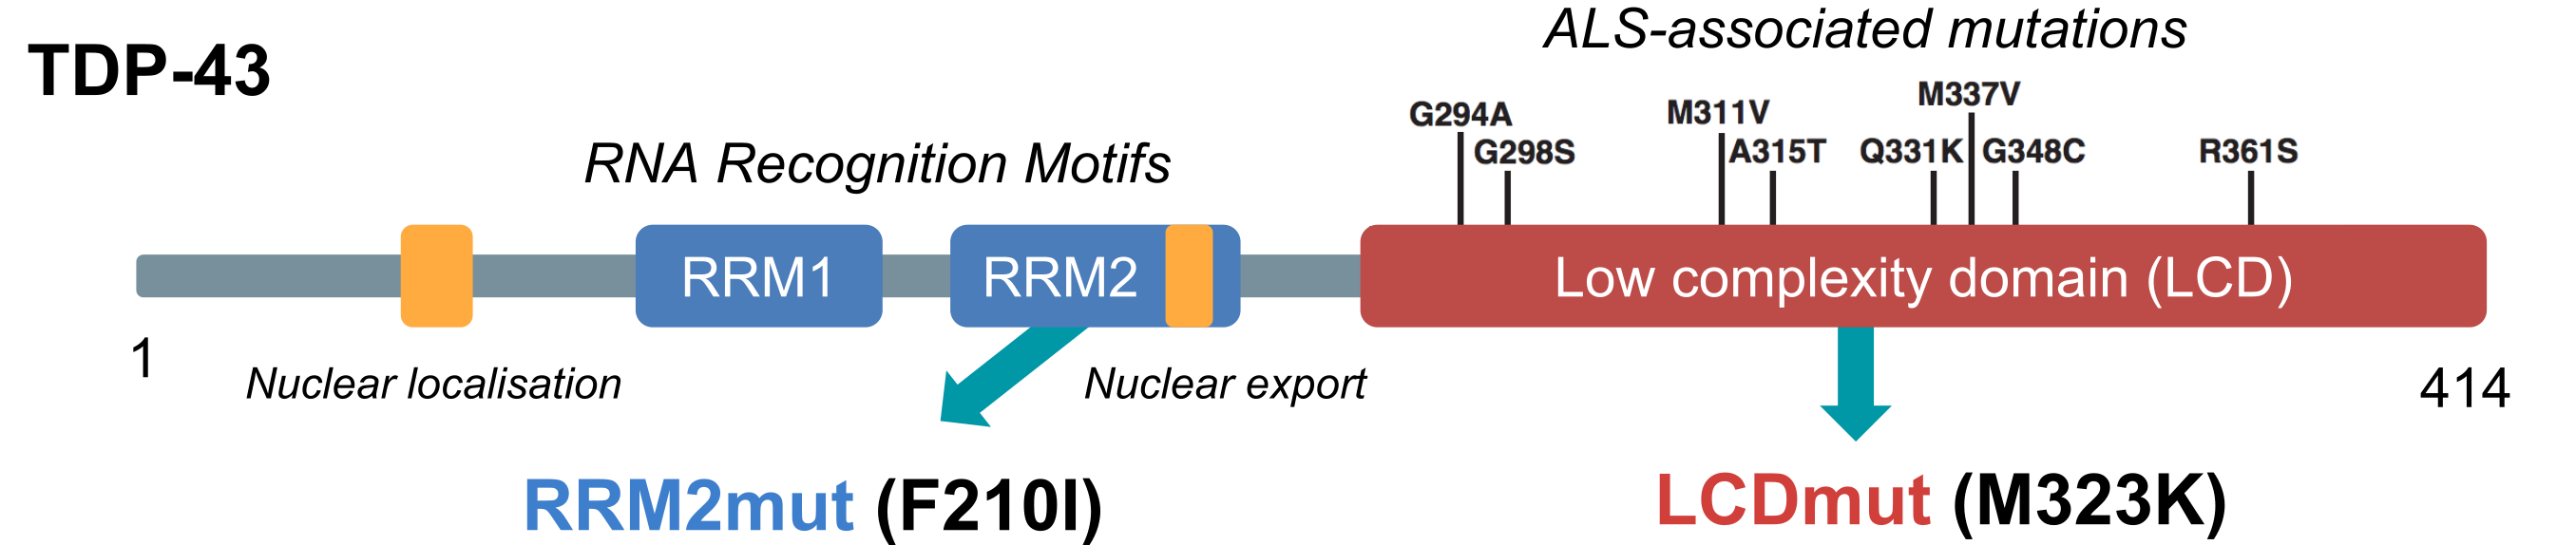
\includegraphics[scale=0.6]{Figures/05_tdp_mice/TDP_structure_mutations.png}
	%\end{center}
	\caption{Two TARDBP mutations and their location within the TDP-43 protein}
	RRM2mut affects the second RNA recognition motif whereas LCDmut affects the C-terminal low complexity domain.
	\label{fig:tdp_structure}
\end{figure}

N-ethyl-N-nitrosourea (ENU) is a very potent mutagenic compound. Dosing male mice with ENU induces point mutations in sperm cells \citep{DeAngelis2000}. Large banks of mutant mouse sperm are maintained at MRC Harwell \citep{Acevedo2008} and the RIKEN in Japan \citep{Gondo2010}. From these resources two mouse lines with mutations in \textit{Tardbp} were chosen, F210I and M323K. The F210I mutation lies within the second RNA recognition motif (RRM2) of the TDP-43 protein whereas M323K lies within the C-terminal low complexity domain (LCD), the hotspot for ALS mutations (figure \ref{fig:tdp_structure}), and specifically within a 20 amino acid alpha-helical region previously found to be important for liquid phase separation and protein aggregation \citep{Conicella2016}. Developing these two mice allowed us to interrogate TDP-43 function and compare a mutation that would be predicted to impair the RNA binding ability of TDP-43 (F210I) with a mutation that potential resembles ALS (M323K). In light of their positions within the protein, the two mutations will be henceforth referred to as RRM2mut and LCDmut respectively.


% info on breeding - F210I is embryonic lethal
Deriving mice from the mutant sperm and backcrossing for several generations onto a mixed C57BL/6J - DBA/2J background revealed that RRM2mut is embryonic lethal in the homozygous state but not in heterozygosity, whereas LCDmut mice are viable and live normal lifespans. However, close observation of aged LCDmut revealed gradual muscle weakness and a reduction in motor neuron numbers in the spinal cord (data not shown), suggesting that the patient-like M323K mutation indeed causes symptoms of neurodegeneration reminiscent of ALS. 

\subsection{The two mutations have opposing effects on splicing known TDP-43 targets}


\begin{figure}[h!]
	%\begin{center}
	\centering
	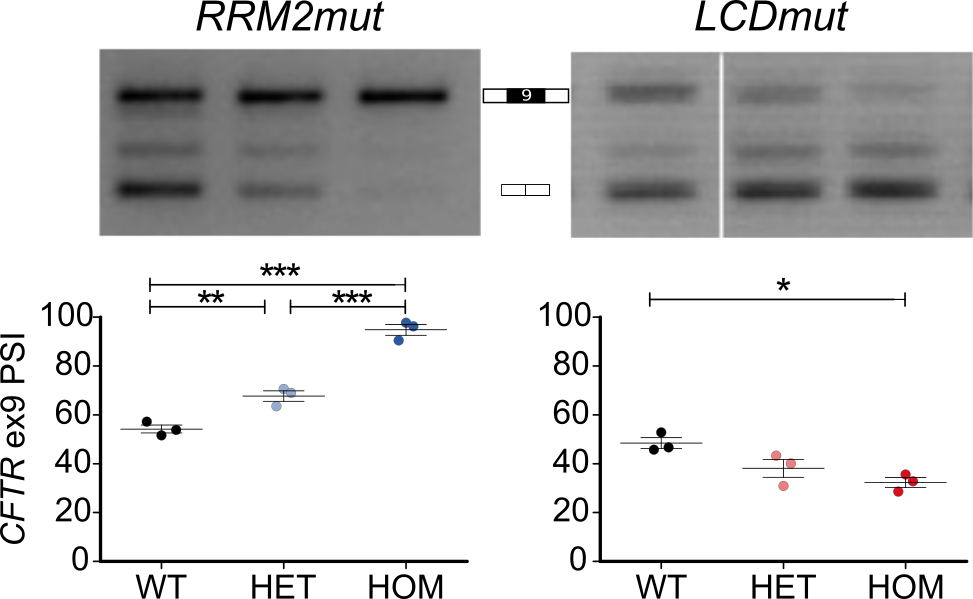
\includegraphics[width=12cm]{Figures/05_tdp_mice/CFTR.png}
	%\end{center}
	\caption{Opposite effects on splicing CFTR exon 9 minigene, a known TDP-43 splicing target}
	RT-PCR traces from primers flanking CFTR exon 9, quantified as PSI ratios for each genotype. *** P < 0.0001 (ANOVA); ** P < 0.01; *** P < 0.001 (Tukey post-hoc test)	
	\label{fig:CFTR}
\end{figure}

Exon 9 of the \textit{CFTR} gene was the first splicing target of TDP-43 to be described in the literature \citep{Buratti2001-et}, as knocking down TDP-43 leads to increased exon 9 inclusion, suggesting that TDP-43 acts to promote exon skipping at this site. We made use of a minigene construct created from \textit{CFTR} exon 9 and its two flanking exons  \citep{Buratti2007minigene}.   Reverse-Transcriptase Polymerase Chain Reaction (RT-PCR) was performed to amplify between primers that flank exon 9. Analysis of the gel electrophoresis traces shows two bands: a larger band corresponding to exon 9 inclusion and a smaller band corresponding to exon 9 skipping. The ratio of inclusion over skipping was calculated for RRM2mut and LCDmut and shown in figure \ref{fig:CFTR}. RRM2mut has a clear dose-dependent increase in exon 9 inclusion and thus resembles a loss of TDP-43 function. Conversely, LCDmut has a dose-dependent increase in exon 9 skipping, suggesting that the pro-skipping action of TDP-43 is increased at this locus and the LCDmut mutation causes a gain of splicing function.


%% INSERT TDP MEF SCATTERS
\begin{figure}[h!]
	\centering
	%\begin{center}
	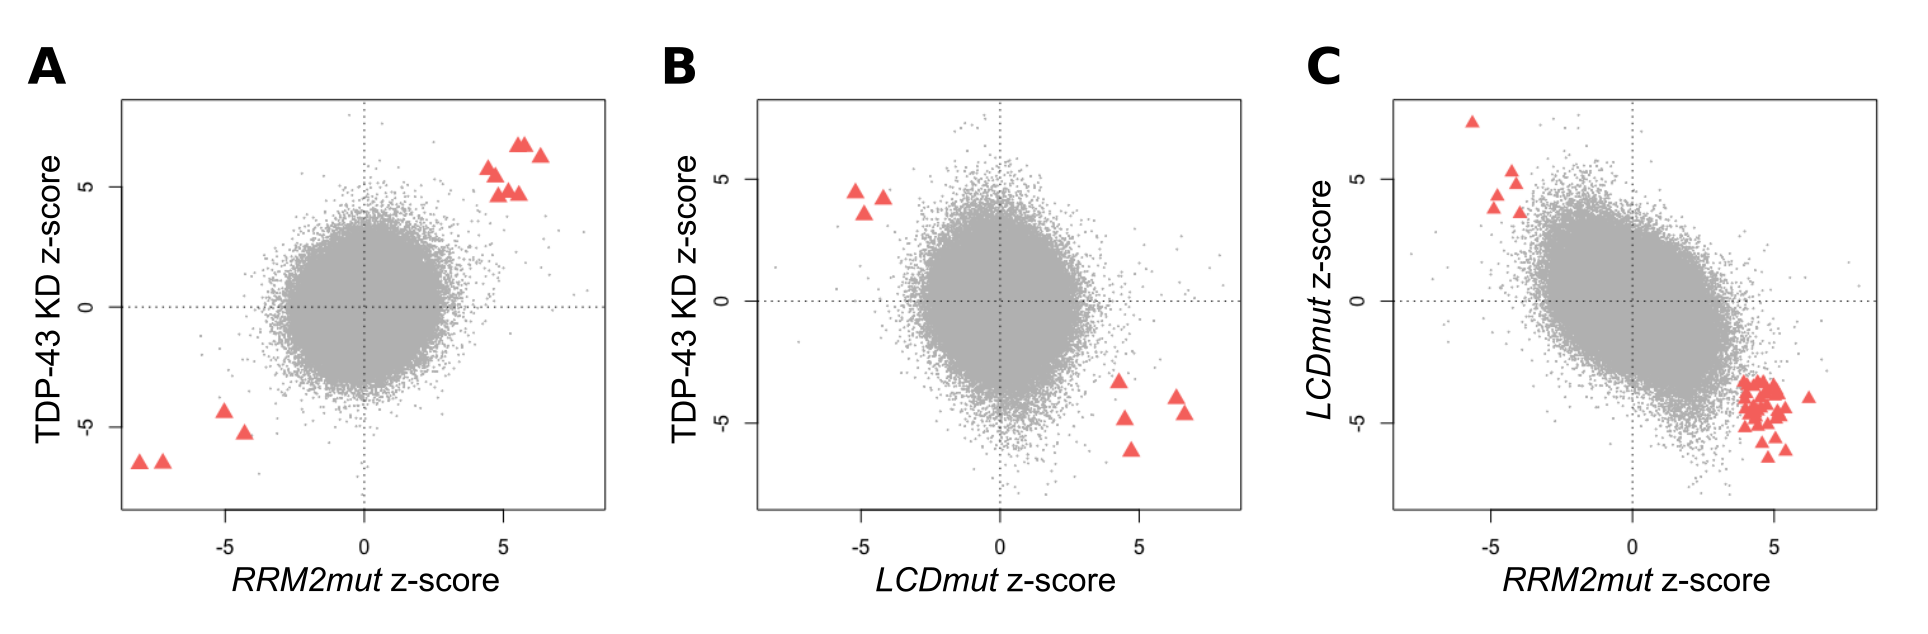
\includegraphics[width=14cm]{Figures/05_tdp_mice/mef_scatters.png}
	%\end{center}
	\caption{\textbf{Comparing the two mutations with a TDP-43 shRNA knockdown}}
	Signed Z-scores for all exons found by DEXSeq in the mouse embryonic fibroblasts, comparing a TDP-43 shRNA knockdown to RRM2mut (A) and LCDmut (B) and comparing the two mutations (C). Exons significant at FDR < 10\% plotted as red triangles, non-significant exons plotted as grey dots.
	\label{fig:mef_scatters}
\end{figure}

To look transcriptome-wide at the effects of the two mutations on simple cassette exon splicing we generated low-depth RNA-seq data from mouse embryonic fibroblasts. To compare both mutations to a simple loss of TDP-43 we employed an short hairpin RNA (shRNA) that targets Tardbp mRNA for degradation, reducing TDP-43 protein levels. A cassette exon splicing analysis was performed in DEXSeq and the fold change and P value from each exon was converted into a signed z-score and two way comparisons were plotted between the shRNA knockdown of TDP-43 (TDP-KD), LCDmut and RRM2mut (figure \ref{fig:mef_scatters}). Separating each graph into quadrants makes it clearly apparent that all significantly changed exons found in each mutation are changed in the same direction between RRM2mut and TDP-KD, and in the opposite direction between LCDmut and TDP-KD, as well as between LCDmut and RRM2mut. This provides evidence at transcriptome scale that the RRM2mut is equivalent to a loss of TDP-43 function and LCDmut is behaving oppositely.

\subsection{RRM2mut leads to a loss of splicing function and cryptic exons}

%%CASSETTE EXON SCATTERS
\begin{figure}[h!]
	\centering
	%\begin{center}
	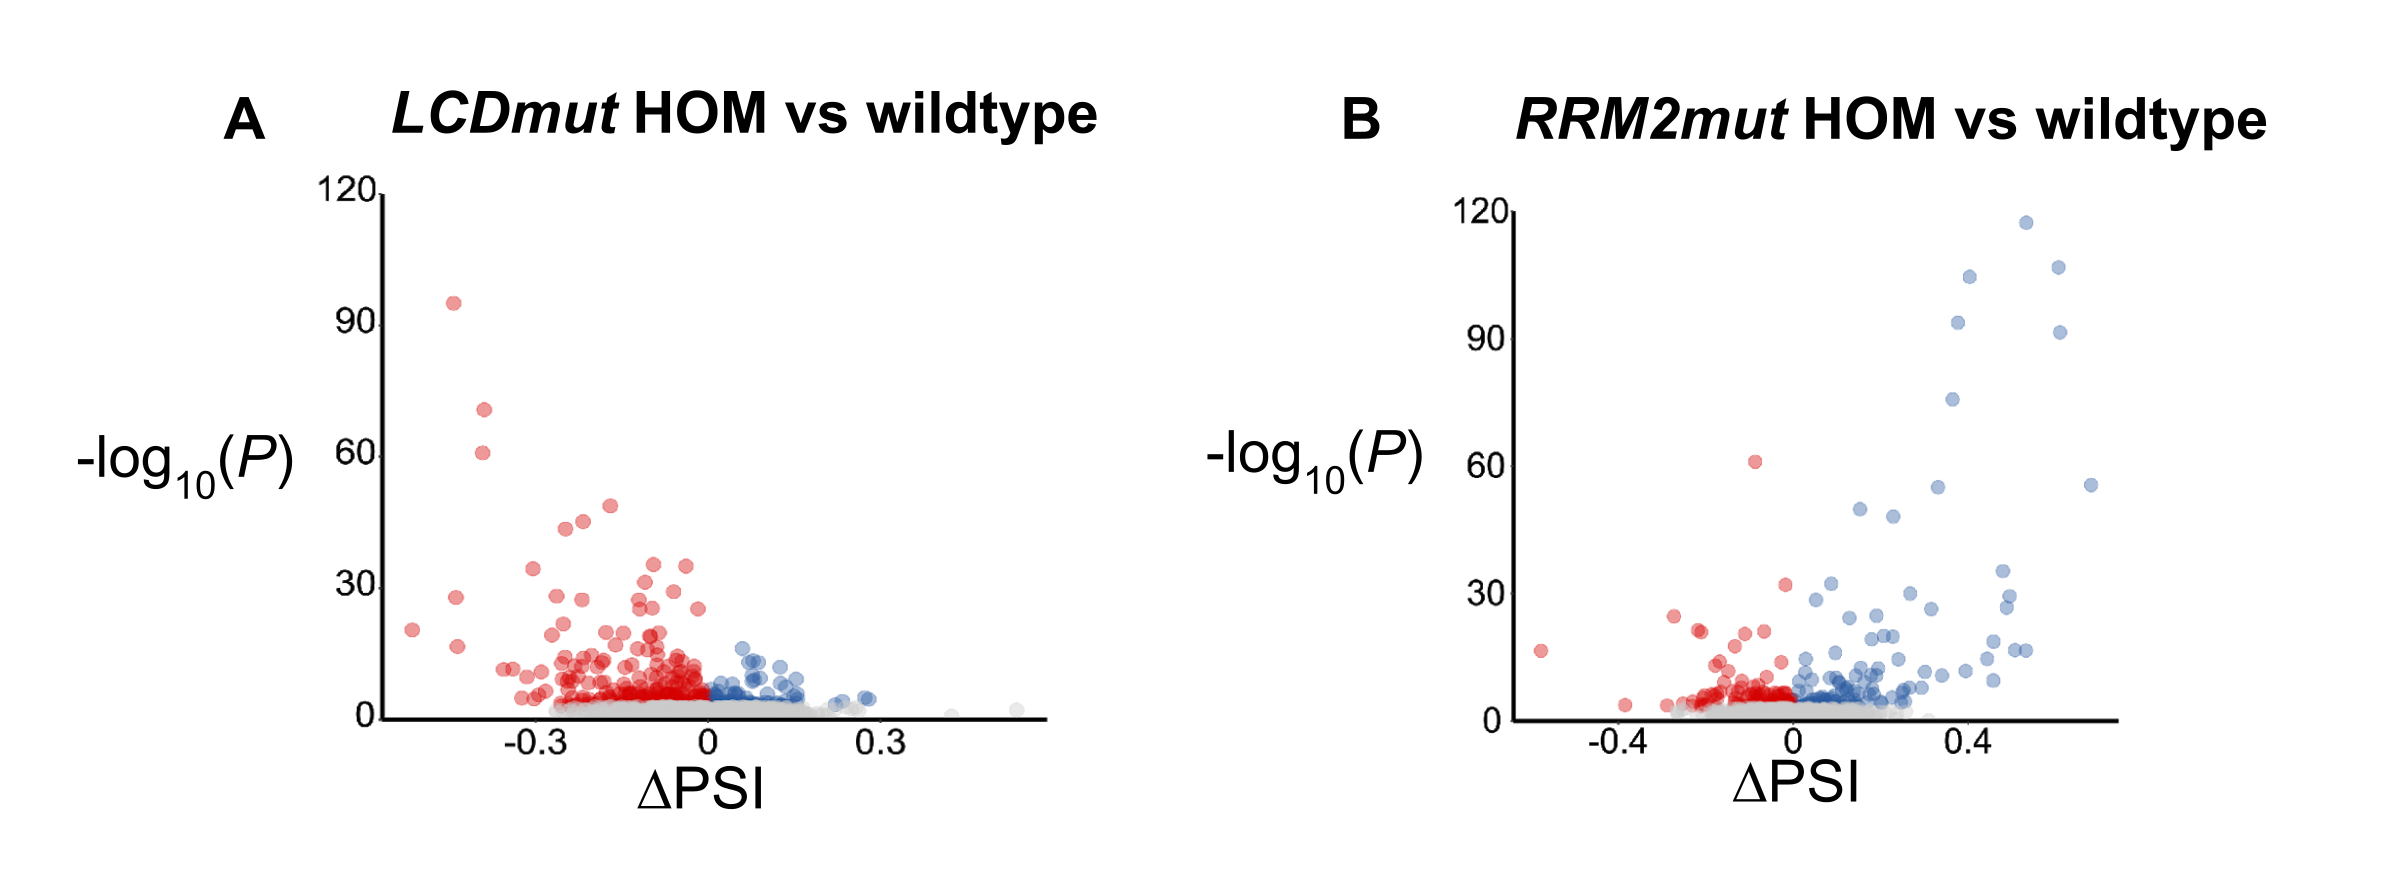
\includegraphics[width=18cm]{Figures/05_tdp_mice/transcriptome_scatters.png}
	%\end{center}
	\caption{\textbf{Direction of cassette exon splicing in the two mutant lines}}
	All splicing events found by SGSeq plotted by p-value and direction ($\Delta$PSI; see methods) for LCDmut (A) and RRM2mut (B).
	\label{fig:cassette_scatters}
\end{figure}

To deeply interrogate splicing changes at time points that were relevant to the phenotypes of interest (death in RRM2mut and neurodegeneration in LCDmut) we generated high depth RNA-seq from RRM2mut embryonic brains and LCDmut adult brains (30 days post-natal ???). High depth and longer read data allows for better discrimination of novel splicing events and so we ran a novel splicing analysis using SGSeq. Plotting the direction and P-value of all cassette exons found in the two mutations strongly suggests that the most striking splicing changes are in exon inclusion in RRM2mut and in exon skipping in LCDmut (figure \ref{fig:cassette_scatters}).

%% CRYPTIC EXONS IN RRM2mut
\begin{figure}[h!]
	\begin{center}
		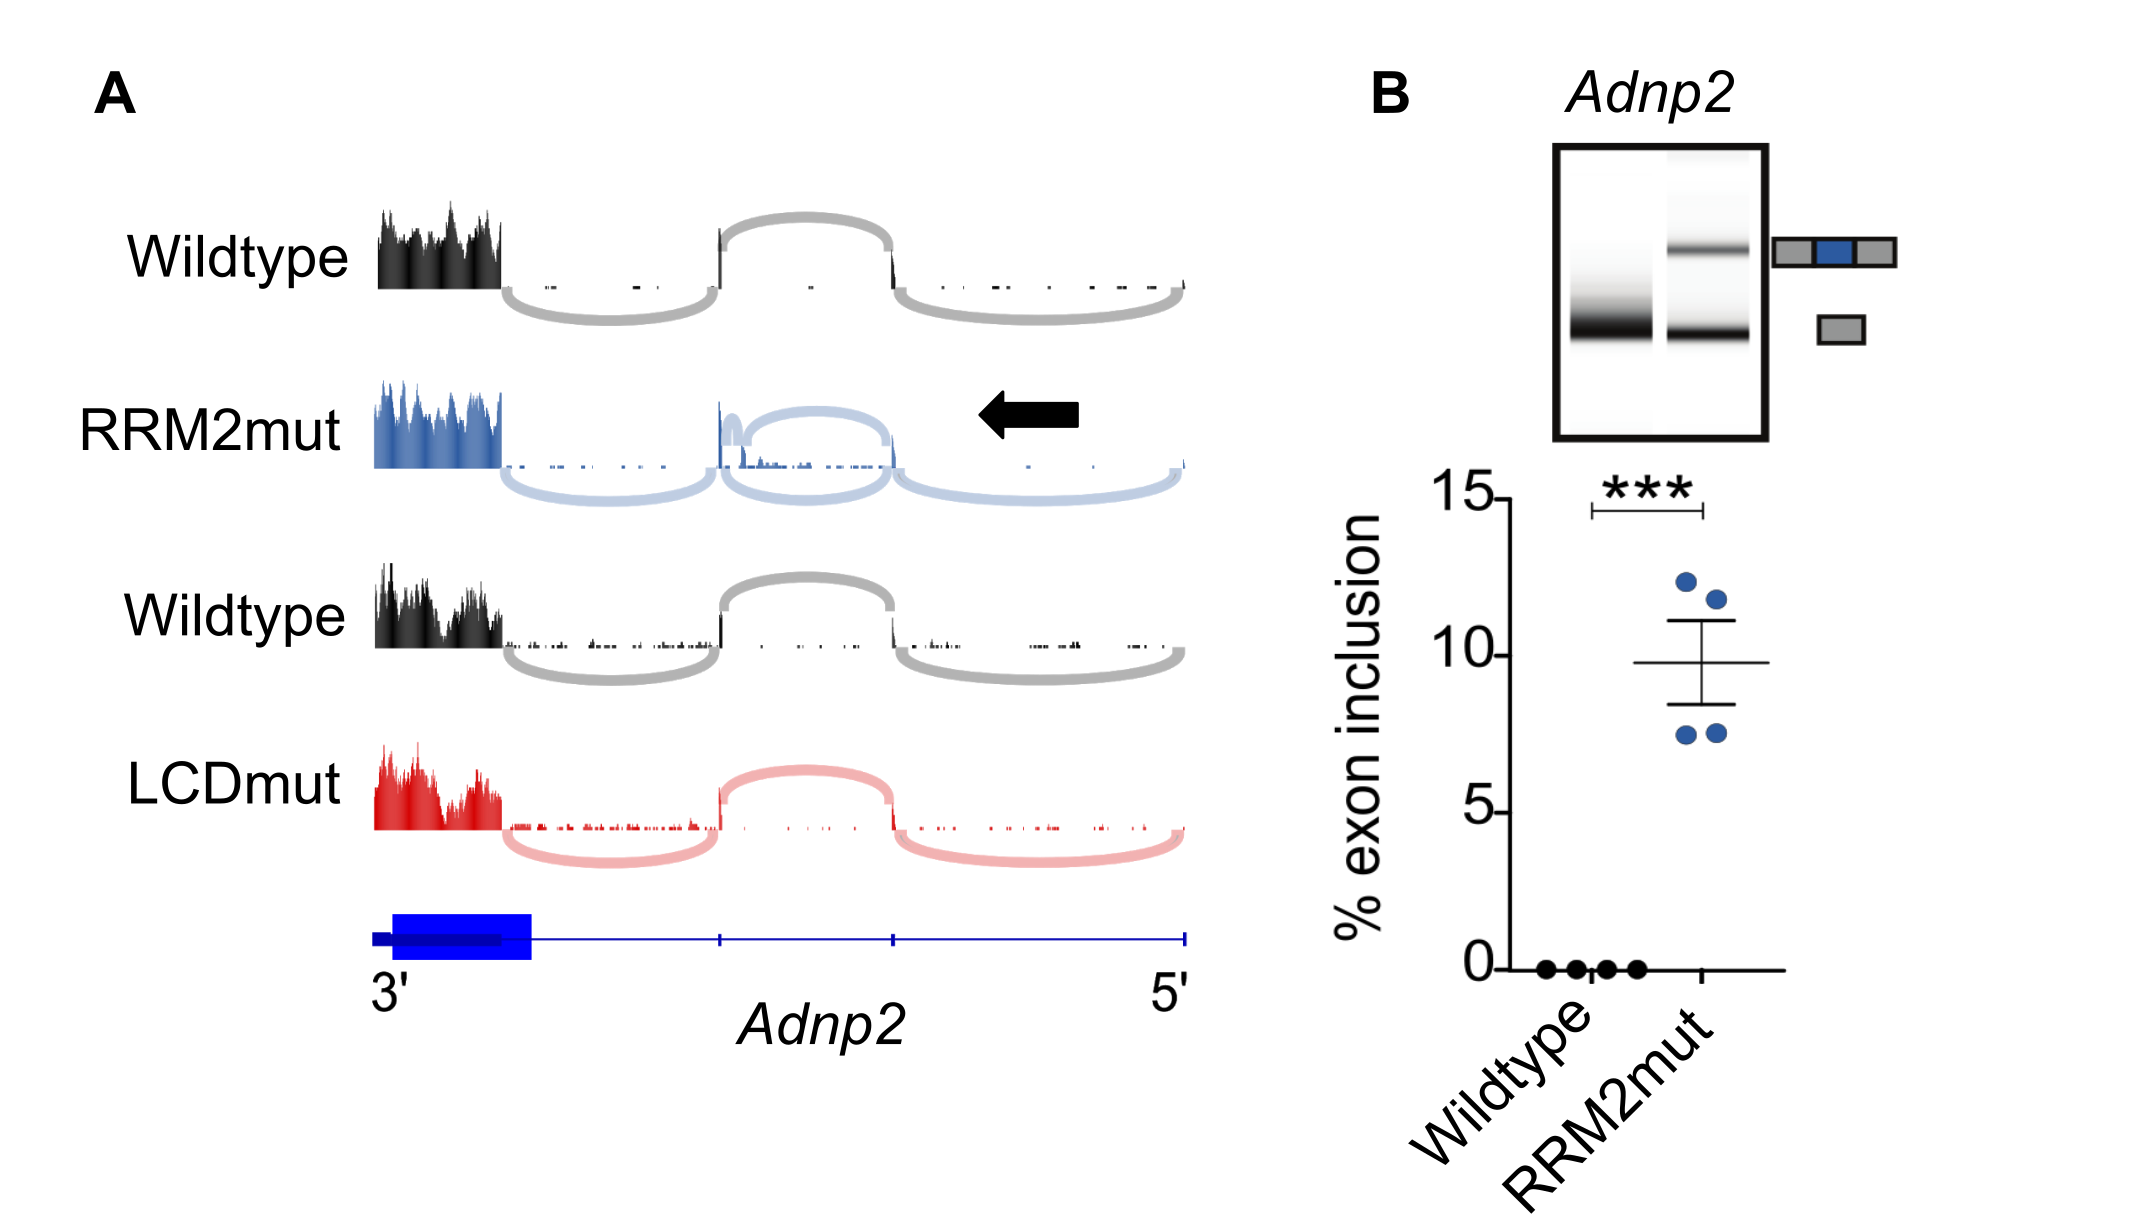
\includegraphics[width=14cm]{Figures/05_tdp_mice/cryptic_exon_multi.png}
	\end{center}
	\caption{\textbf{RRM2mut leads to cryptic exon splicing}}
	\label{cryptic_multi}
	A: Representative RNA-seq traces show cryptic exon in \textit{Adnp2} included in RRM2mut specifically. B: RT-PCR of \textit{Adnp2} selectively amplifies a band corresponding to cryptic exon inclusion in RRM2mut samples. P < 0.001; t-test(two-sided). C: PhyloP conservation scores for 1000 randomly chosen mouse exons compared to the 33 cryptic exons found in RRM2mut.
\end{figure}

A hallmark of TDP-43 depletion is the widespread inclusion of non-conserved cryptic exons \citep{Ling2015}. Rather than relying on isoform annotation we filtered all cassette exons found in RRM2mut and selected those that were barely or not at all spliced in wildtypes but we included in RRM2mut samples, resulting in 33 candidate cryptic exons being discovered. A representative example of a cryptic exon in \textit{Adnp2} is shown in figure \ref{cryptic_multi}, changing from 0\% inclusion in wildtype mice to ~10\% inclusion in RRM2mut but not in LCDmut mice.  

%% LONG GENES 
\begin{figure}[h!]
	\begin{center}
		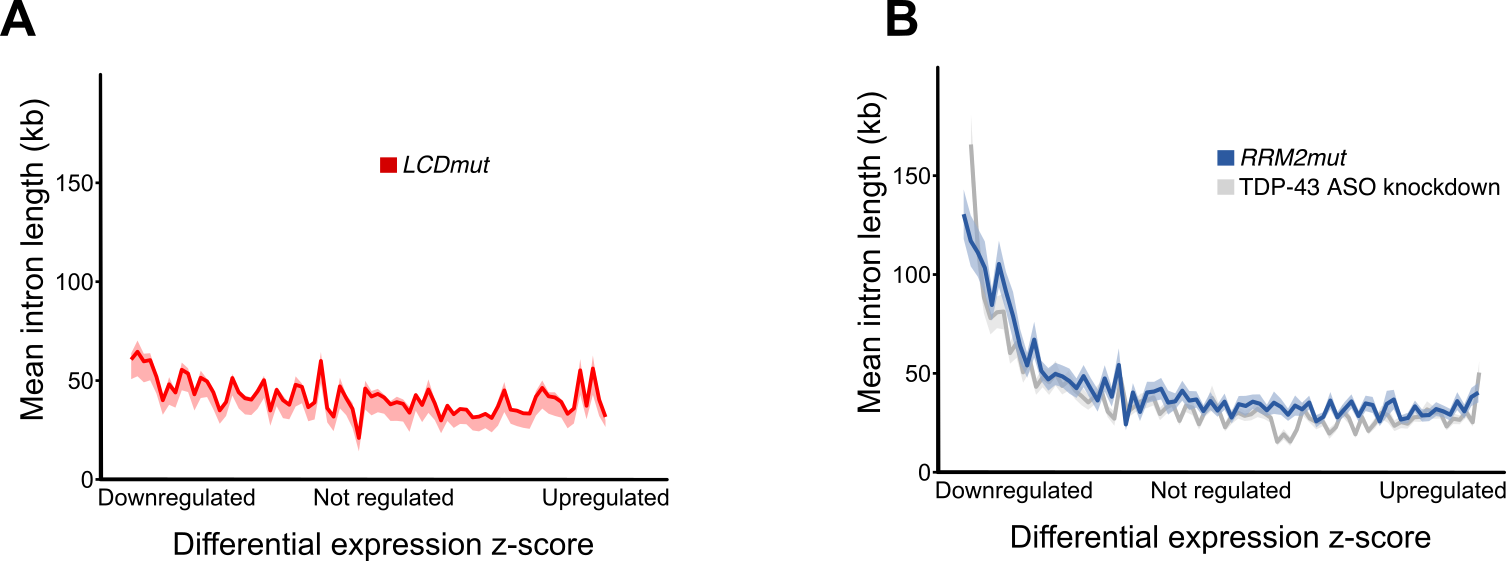
\includegraphics[width=14cm]{Figures/05_tdp_mice/long_genes.png}
	\end{center}
	\caption{\textbf{RRM2mut gene expression has bias for long gene downregulation, mirroring TDP-43 knockdown data}}
	Mean intron length in kilobases for bins of genes ordered by signed Z-score. TDP-43 antisense olignucleotide (ASO) knockdown data taken from \cite{Polymenidou2011-hs}.
	\label{fig:long_genes}
\end{figure}

%% LONG GENES iCLIP
\begin{figure}[h!]
	\begin{center}
		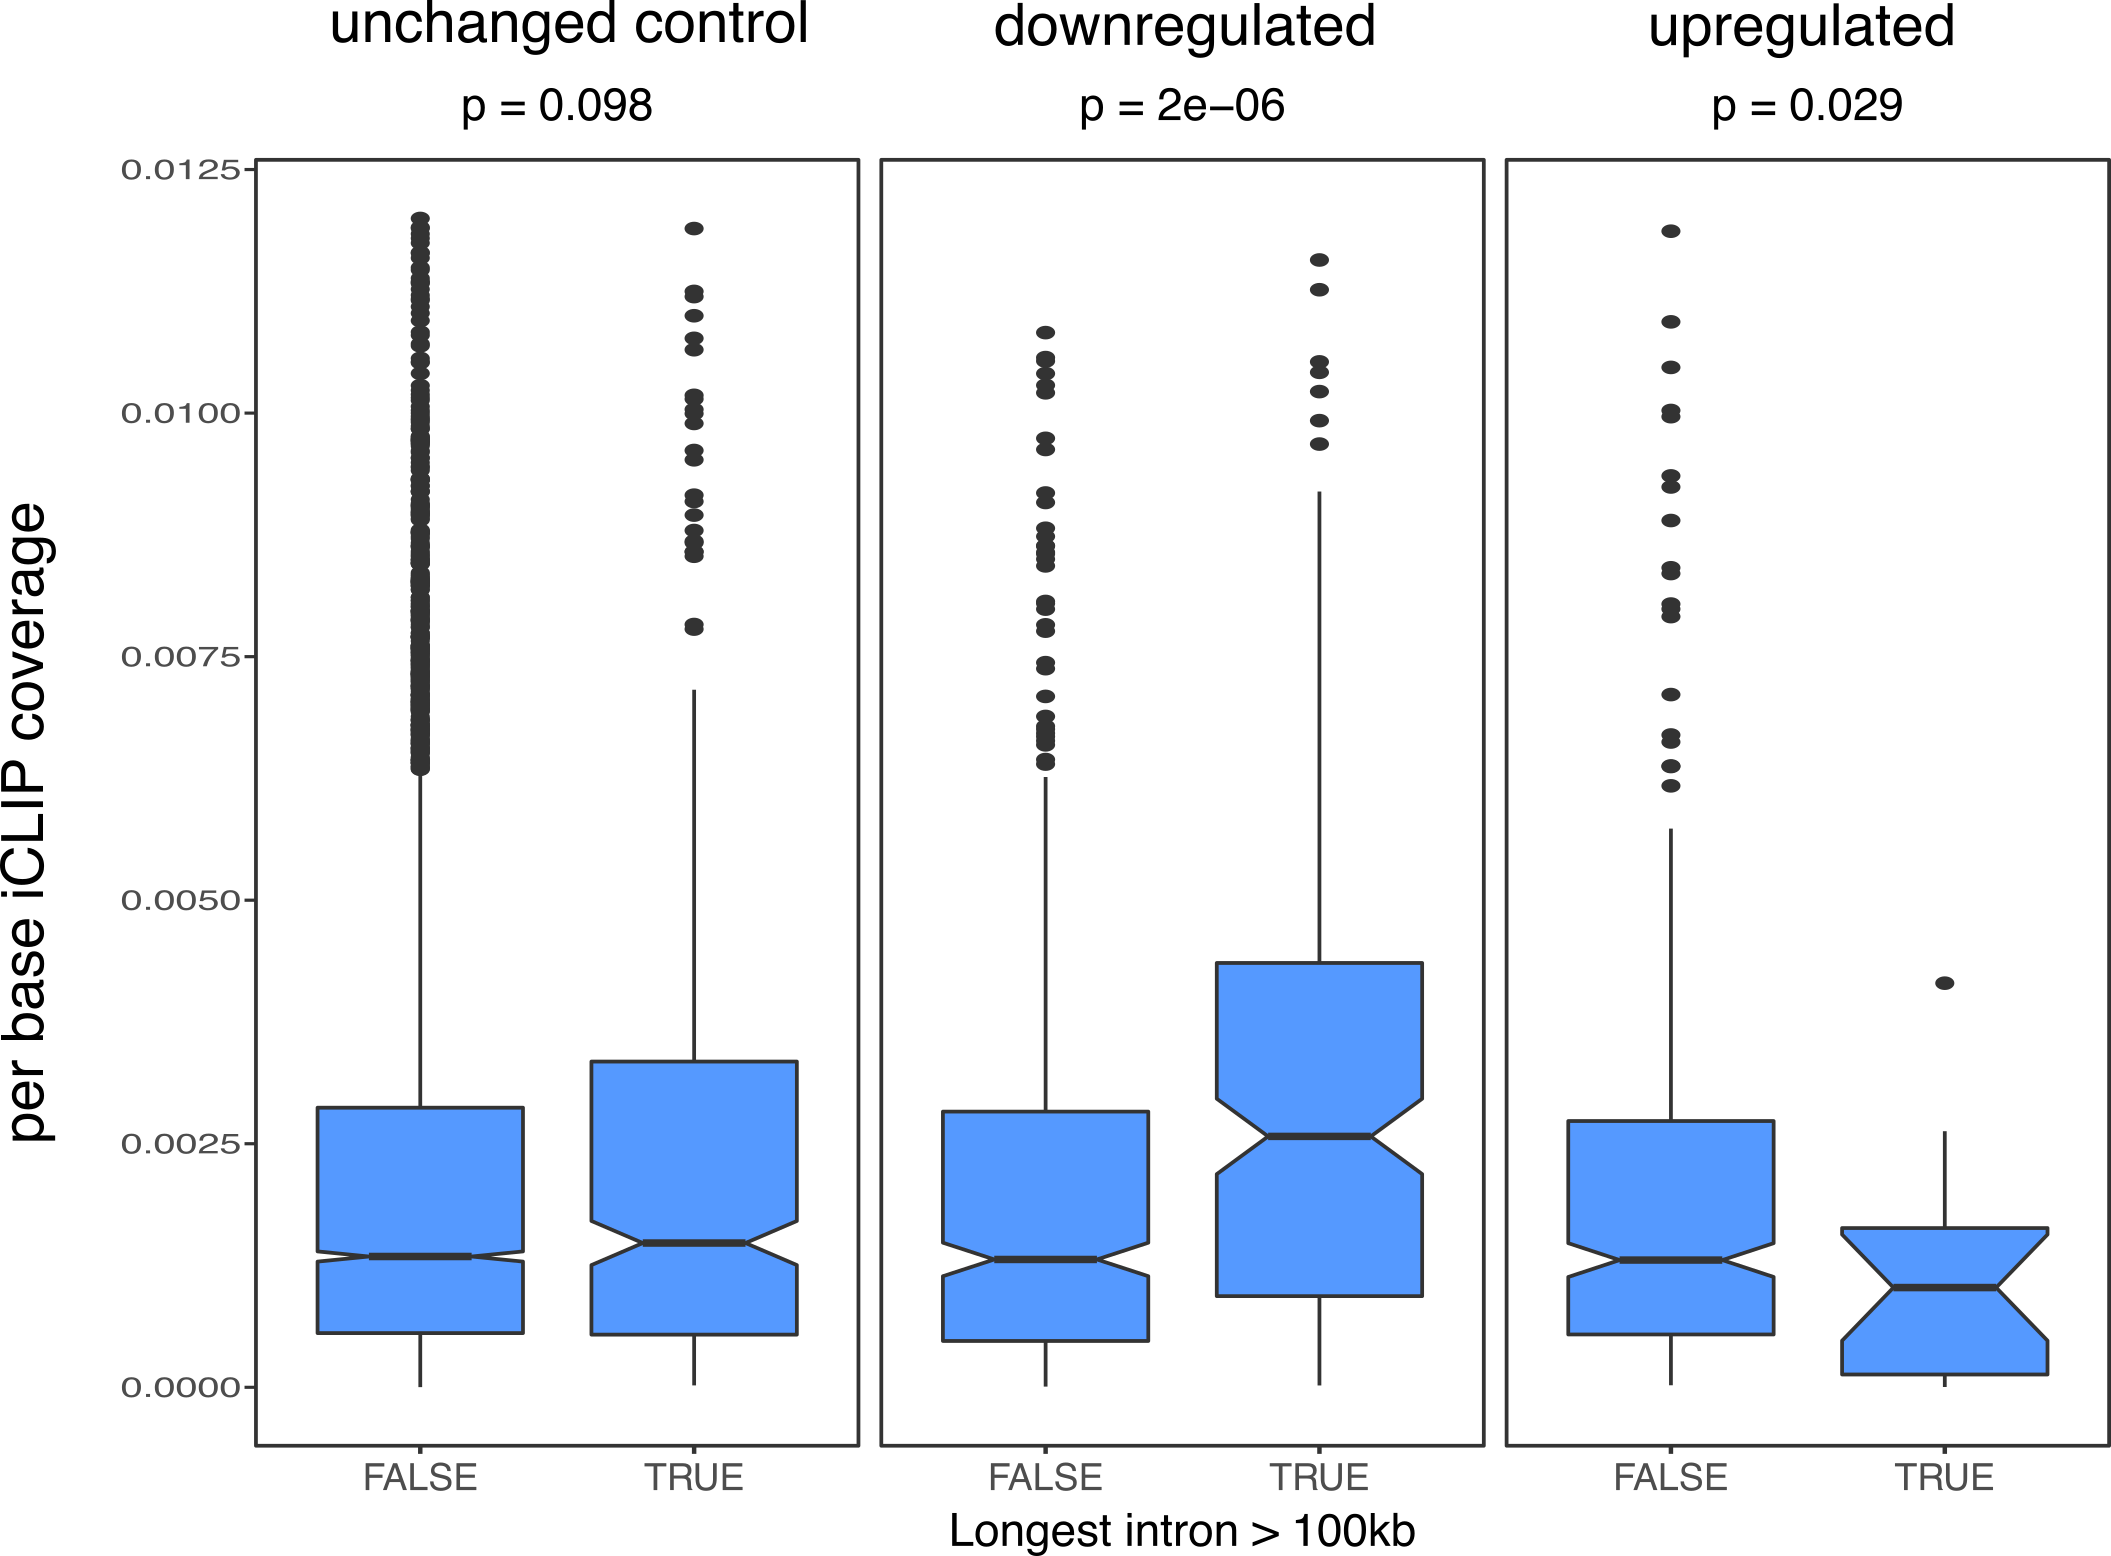
\includegraphics[width=14cm]{Figures/05_tdp_mice/long_genes_iclip.png}
	\end{center}
	\caption{\textbf{RRM2mut downregulated long genes are enriched for TDP-43 iCLIP binding}}
	The per-nucleotide overlap of iCLIP interaction peaks for each gene is significantly increased in long intron genes downregulated in RRM2mut mice compared to wildtype. P values are from Mann-Whitney-Wilcoxon test.
	\label{fig:long_genes_iclip}
\end{figure}



Another feature of TDP-43 loss of function is a striking downregulation of genes with long introns (>100kb). This phenomenon was first observed in mice where an antisense oligonucleotide strategy was used to lower TDP-43 in the striatum (TDP-ASO); \citep{Polymenidou2011-hs}. Long intron genes are particularly prevalent in neuronal cells and it is thought that TDP-43 binds within these long introns to promote their processing and splicing. We re-analysed RNA-seq data from this study and compared it to the RRM2mut and LCDmut sequencing data. Differential gene expression analysis was run and genes were ranked by their direction of expression change between controls and ASO treatment/mutations. Genes were then binned into groups and the lengths of longest intron in each gene were extracted from GENCODE annotation. While in LCDmut, gene length is evenly distributed between downregulated, unchanged and upregulated genes, there is a clear bias for the most downregulated genes having long introns being downregulated in both RRM2mut and TDP-ASO (figure \ref{fig:long_genes}). 
An orthogonal approach is to look at TDP-43 protein-RNA interaction data performed on wildtype cells with the iCLIP method \citep{Huppertz2014-ip}. I calculated the proportion of nucleotides in each gene that had an iCLIP peak overlapping, signifying direct TDP-43 binding. Genes that were downregulated in RRM2mut had no difference in the distribution of iCLIP peak overlaps except for those downregulated genes that also contained at least one intron longer than 100 kilobases (figure \ref{fig:long_genes_iclip}). 


\subsection{LCDmut shows the inverse of cryptic splicing - skiptic splicing}

\begin{figure}[h!]
	\begin{center}
		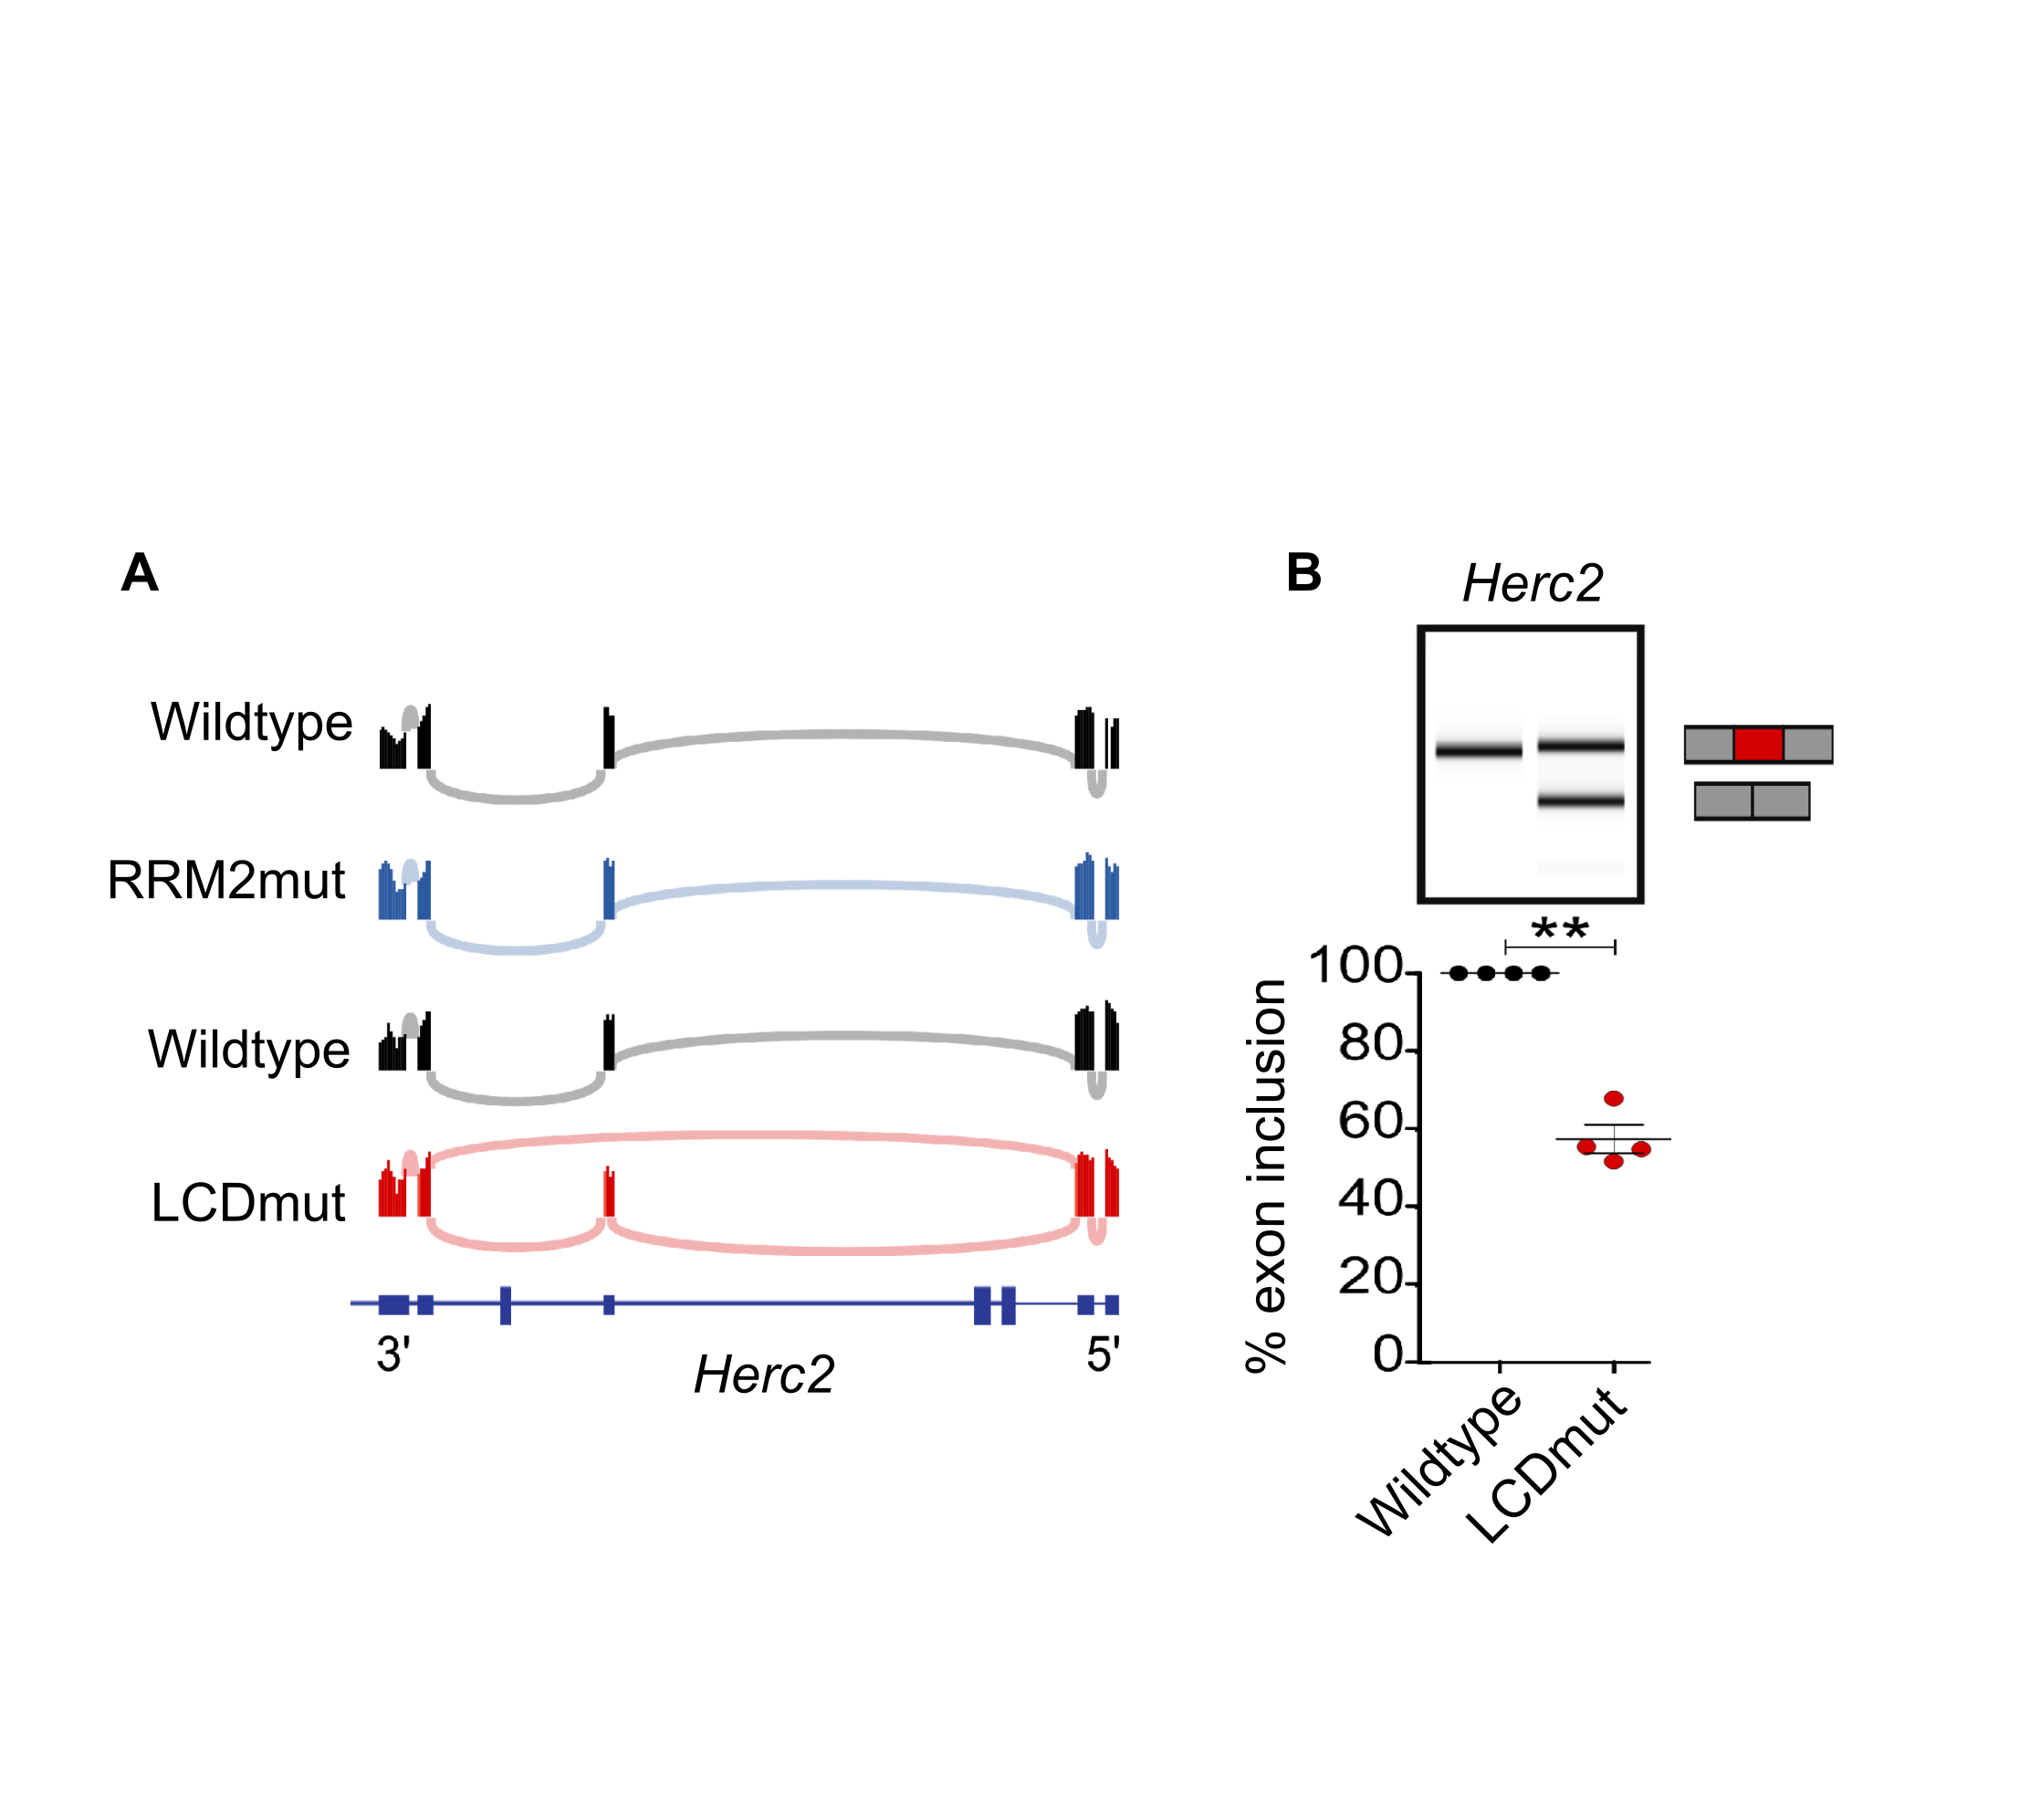
\includegraphics[width=14cm]{Figures/05_tdp_mice/skiptic_exon_multi.png}
	\end{center}
	\caption{\textbf{LCDmut leads to skiptic exon splicing}}
	A: Representative RNA-seq traces show a constitutive exon in \textit{Herc2} skipped in LCDmut specifically - a skiptic exon. B: RT-PCR of \textit{Herc2} selectively amplifies a band corresponding to exon skipping skipping in LCDmut samples. P < 0.001; t-test(two-sided). C: PhyloP conservation scores for 1000 randomly chosen mouse exons compared to the 48 skiptic exons found in LCDmut.
	\label{skiptic_multi}
\end{figure}

We applied the same cryptic exon filtering strategy to LCDmut and found a small number of potential cryptic exons. However, when applying the inverse critera to find exons that are 95-100\% included in wildtype and then skipped in LCDmut we uncovered 48 exons. These exons are constitutively spliced and yet are skipped in the presence of the LCDmut, making them the inverse of cryptic exons. We therefore christened them "skiptic" exons - a portmanteau of cryptic and skipping. A selection of skiptic exons were validated by RT-PCR (figure \ref{fig:skiptic_multi}). 


\begin{figure}[h!]
	\begin{center}
		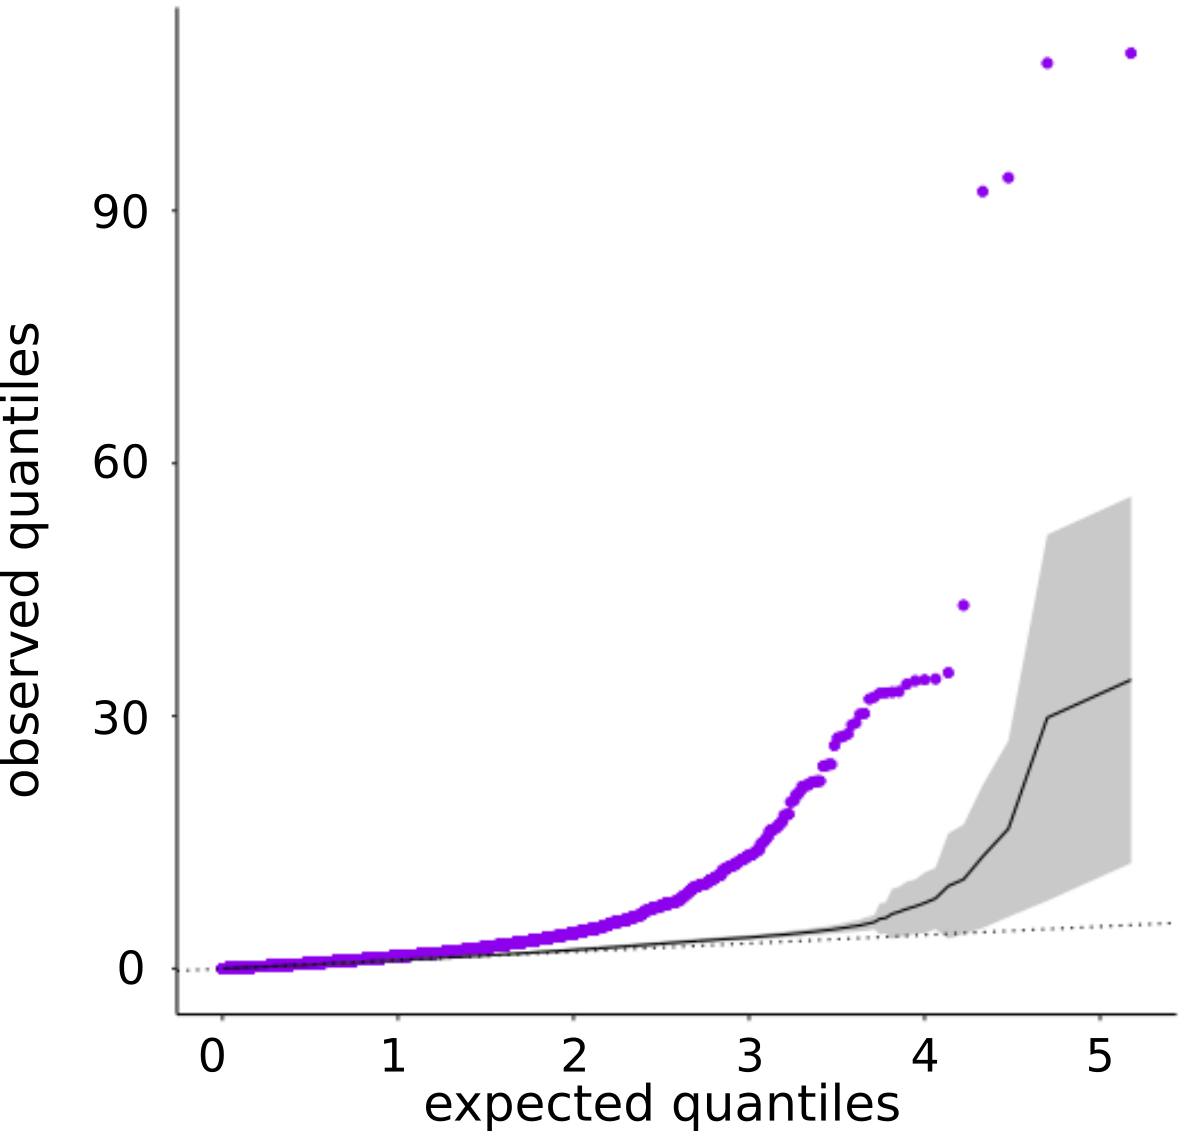
\includegraphics[width=9cm]{Figures/05_tdp_mice/permutation_ribbon.png}
	\end{center}
	\caption{\textbf{Permuting sample order shows clear splicing difference between LCDmut mice from controls}}
	Quantile-quantile plots show the difference between expected and observed distribution of p-values generated from multiple tests. True case-control sample labelling of LCDmut and littermate controls (purple) shows clear inflation of low p-values when compared to all permutations of sample ordering (grey; plotted as mean ± standard deviation).
	\label{fig:permutation}
\end{figure}

To demonstrate that the 48 skiptic exons found in LCDmut were not statistical anomalies due to the small sample size we employed a permutation strategy where the wildtype and LCDmut labels were shuffled 50 times to cover all possible orders and the splicing analysis repeated with the permuted labels. A quantile-quantile plot depicts the distribution of P-values generated in a large set of statistical tests with the theoretical expected distribution. If there is no difference between genotypes then some low p-values are expected by chance due to the small sample size. However, there is a clearly a large difference in splicing between LCDmut and wildtype mice that drives a large inflation in the number of low P-value splicing events far away from the expected null distribution (figure \ref{fig:permutation}).   


\subsection{Both skiptic and cryptic splicing show evidence of direct TDP-43 binding}

\begin{figure}[h!]
	\begin{center}
		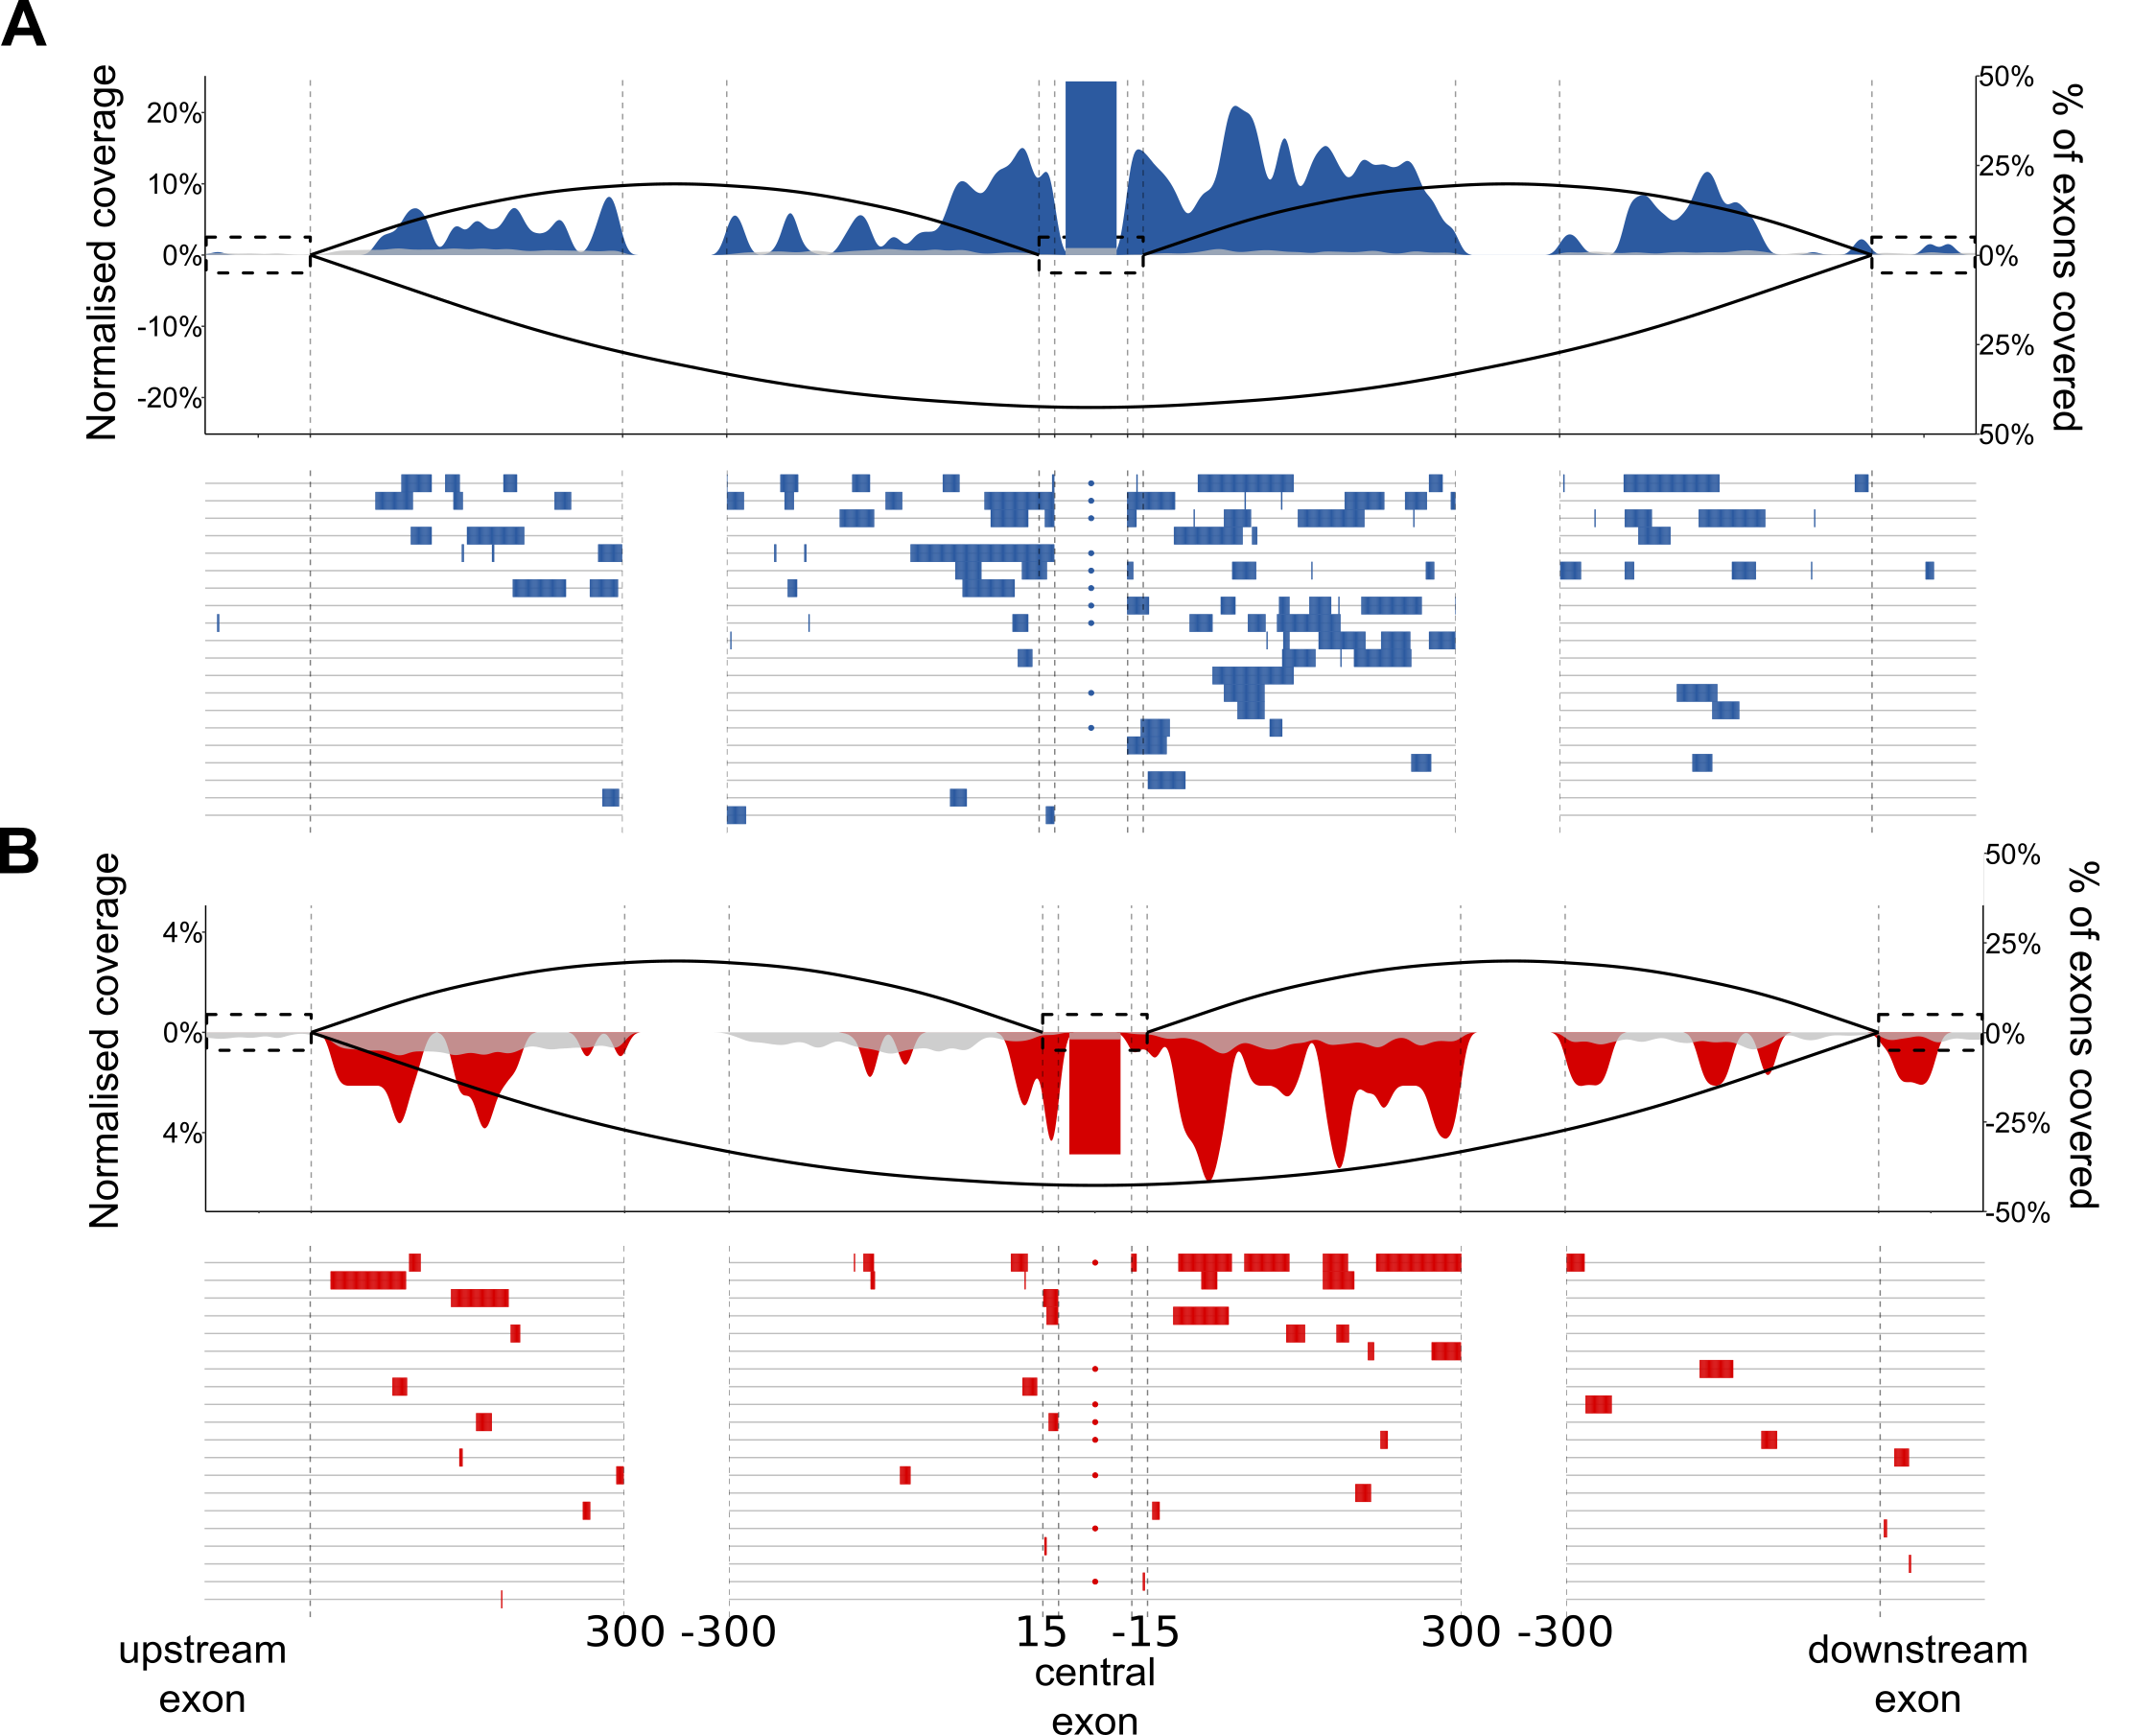
\includegraphics[width=14cm]{Figures/05_tdp_mice/iclip_multipanel.png}
	\end{center}
	\caption{\textbf{RNA maps of skiptic and cryptic exons show direct binding by TDP-43}}
	A: The 33 cryptic exons found in the RRM2mut embryonic mice. Traces show normalised iCLIP peak coverage within and around each exon. Left y-axis: the proportion of exons with an iCLIP peak at that nucleotide. Right y axis: the proportion of central exons or flanking exons that overlap any iCLIP peaks. Below, individual positions of iCLIP peaks for the top 20 cryptic exons. Circles in the centre denote whether there are any iCLIP peaks overlapping the central exon. B: as before for the 48 skiptic exons found in the LCDmut adult mice.
	\label{iclip_multi}
\end{figure}

\begin{table}
	\begin{footnotesize}
	\begin{tabular}{llll}
		& total &	overlap	& \% \\
		\hline
		All exons in GENCODE vM12 &	744,786	& 37,276 & 5\% \\
		All constitutive exons found in all samples	& 239,897	& 17,828	& 7.4\% \\
		All cassette exons found in all samples &	5,656 &	361	& 6.4\% \\
		Significant cassette exons (FDR < 0.05) between LCDmut and wildtype mice	& 260	& 49 & 18.8\% \\
		Skiptic exons (control PSI > = 0.95; dPSI > = -0.05; FDR < 0.05) & 47 &	31 & 66\% \\
	\end{tabular}
	\end{footnotesize}
	\caption{Proportions of exons with any TDP-43 binding from iCLIP}
	\label{tab:iclip_proportions}
\end{table}

Cryptic exons associated with TDP-43 depletion have been demonstrated to originate from mRNA that is directly bound by TDP-43 itself. This suggests that these splicing changes emerge because TDP-43 can no longer act to repress cryptic exon recognition by the splicing machinery and other factors. We wanted to replicate this experiment in the RRM2mut and extend it to the LCDmut-associated skiptic exons to test whether skiptic exon transcripts are bound by TDP-43 in wildtype cells. We created RNA maps to visualise TDP-43 binding across the cryptic and skiptic exons accompanied by their flanking introns. RNA maps are complex data visualisations that take nucleotide-resolution RNA-protein interaction information generated by iCLIP \citep{Huppertz2014-ip}.For the 300bp surrounding the central and flanking exons, the per-nucleotide coverage was normalised as a proportion across all genes tested. For the central exons, due to differences in exon length, the proportion of exons that had any iCLIP information covering them was recorded as a proportion of the total. For comparison, 1000 exons rNA % FINISH

\subsection{Skiptic splicing is predicted to be deleterious to gene expression}

\begin{figure}[h!]
	\begin{center}
		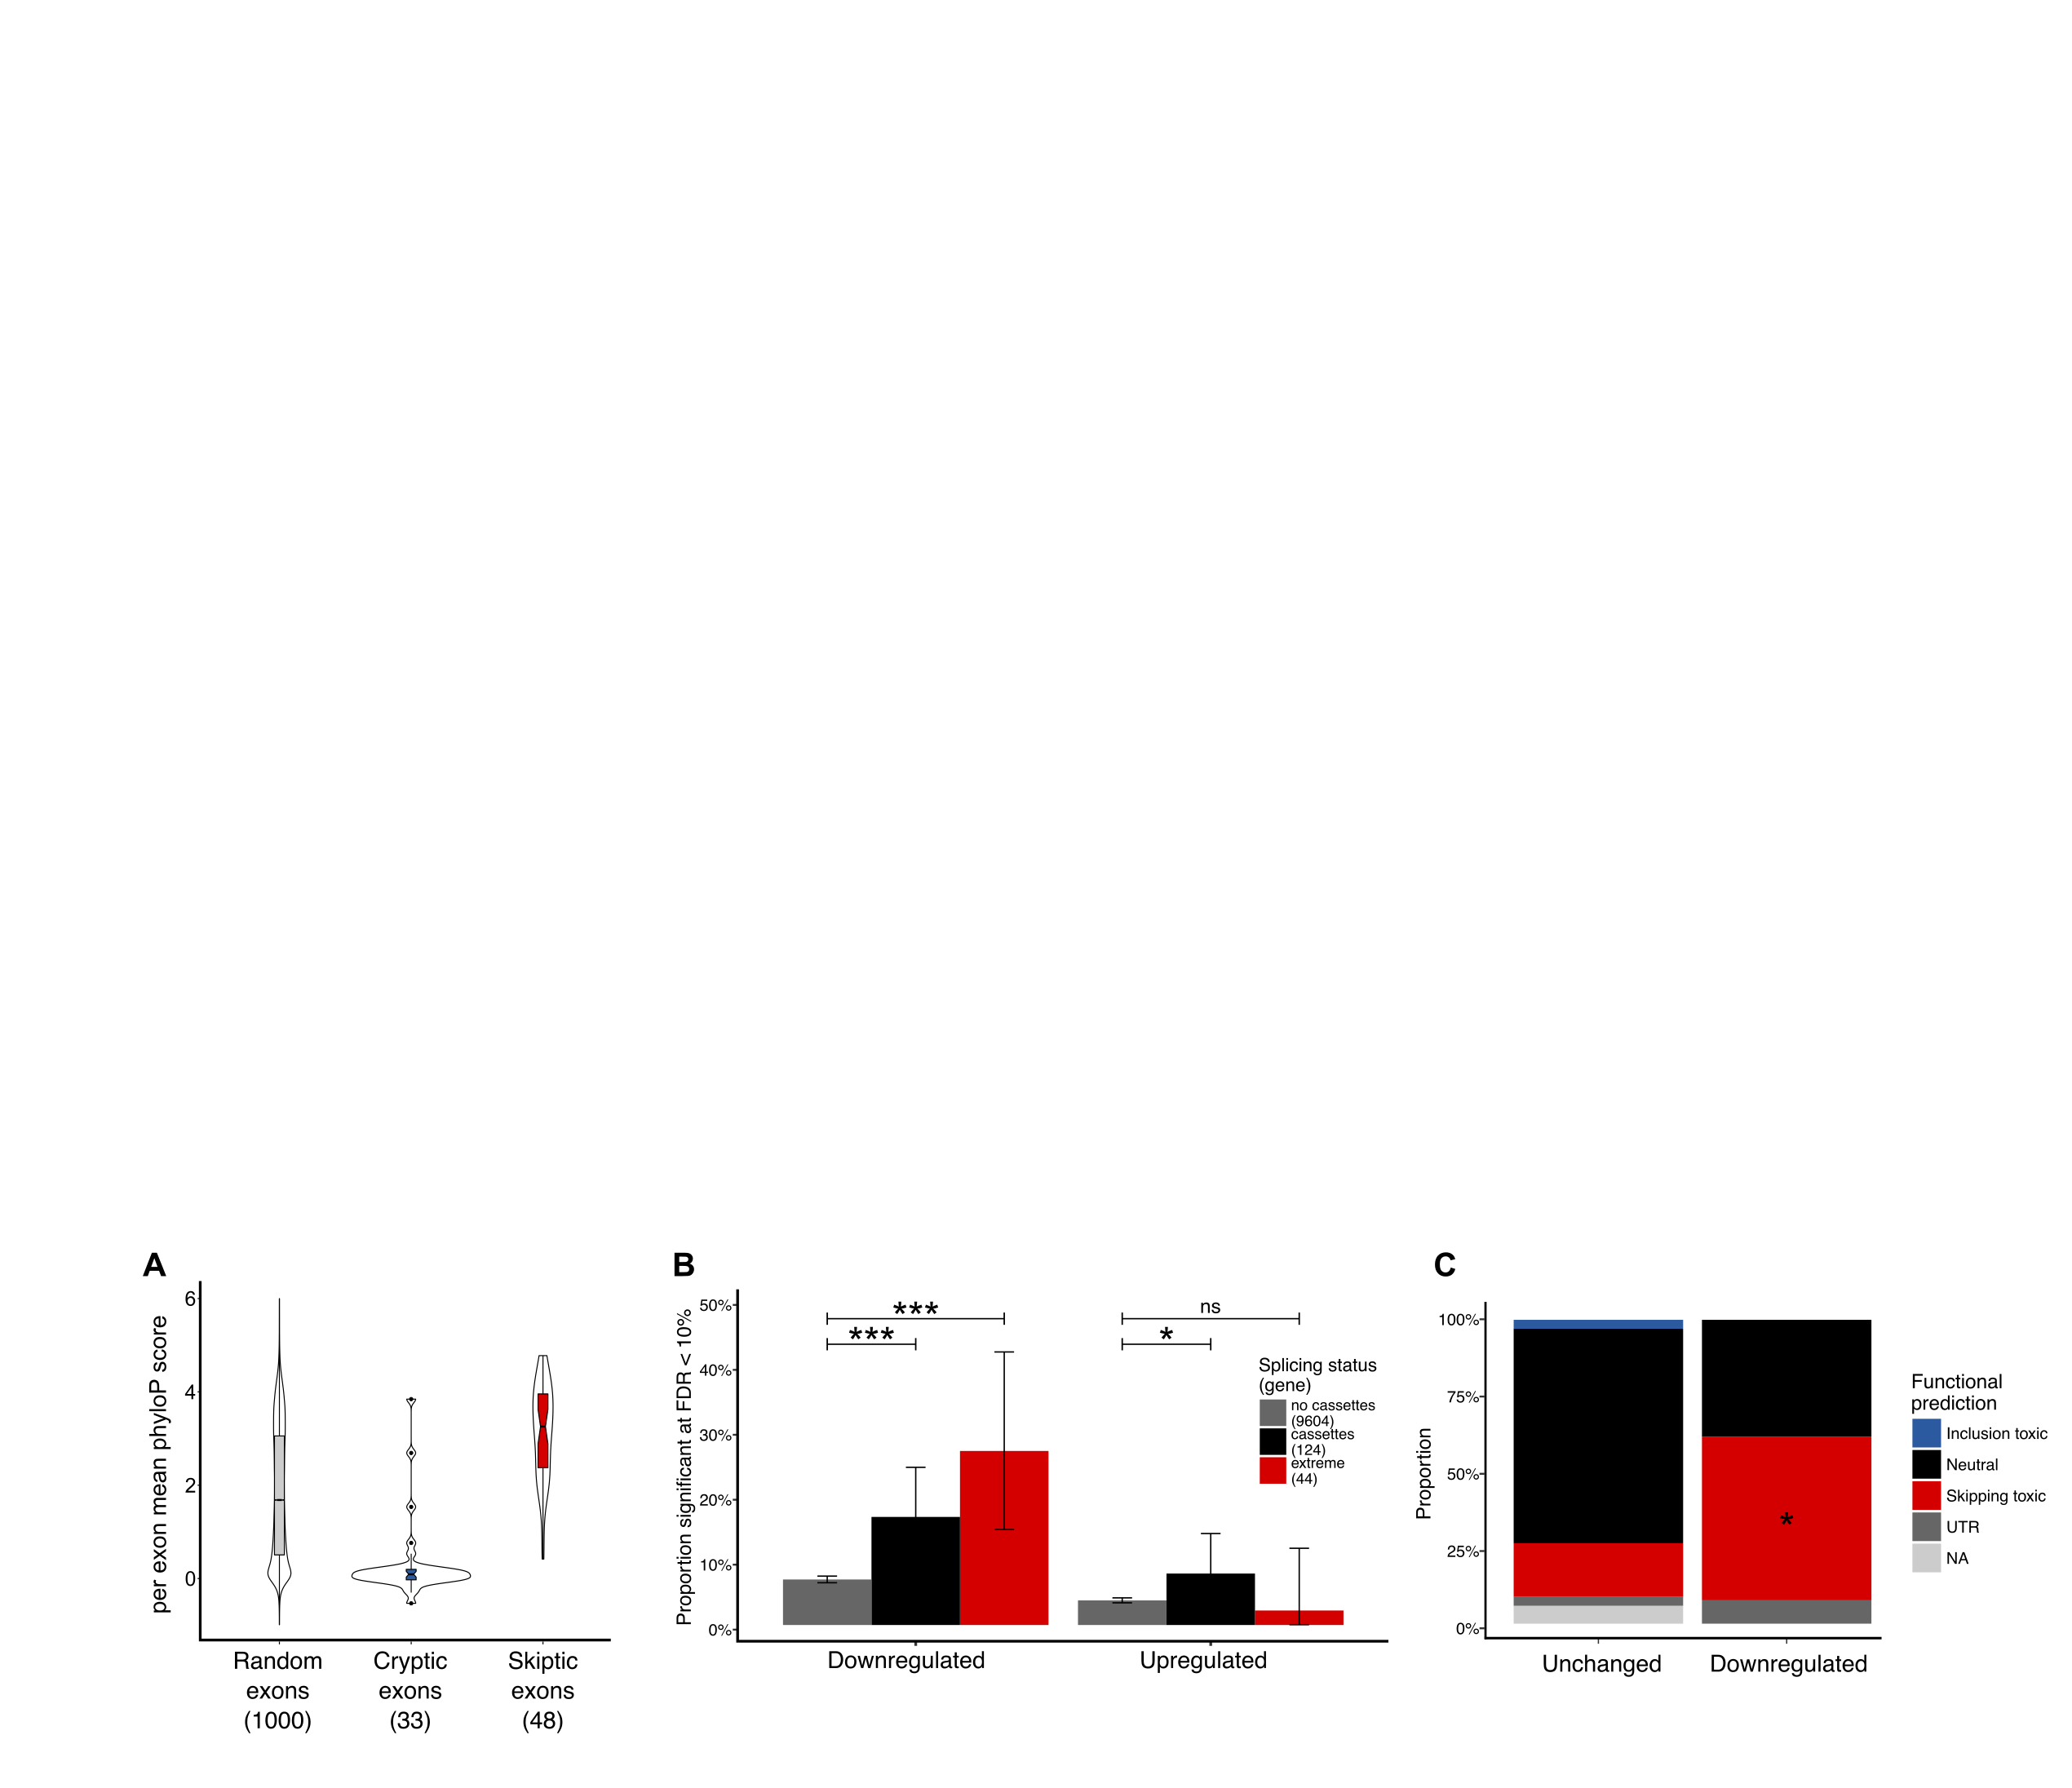
\includegraphics[width=18cm]{Figures/05_tdp_mice/functional_plots.png}
	\end{center}
	\label{functional_plots}
	\caption{\textbf{Functional analyses of the skiptic exons}}
	A: PhyloP conservation scores presented as the mean for each exon. B: proportions of each gene that are either downregulated or upregulated at FDR < 10\%. C: Proportions of predicted downstream consequence of exon skipping for either non-regulated or downregulated skiptic exons. *: P < 0.05; **: P > ??? ***: P < ????
\end{figure}


\subsection{Skiptic splicing can be observed in human ALS patients}
% work performed by Pras - show RT-PCRs
% explain dodgy quantification
\begin{figure}[h!]
	\begin{center}
		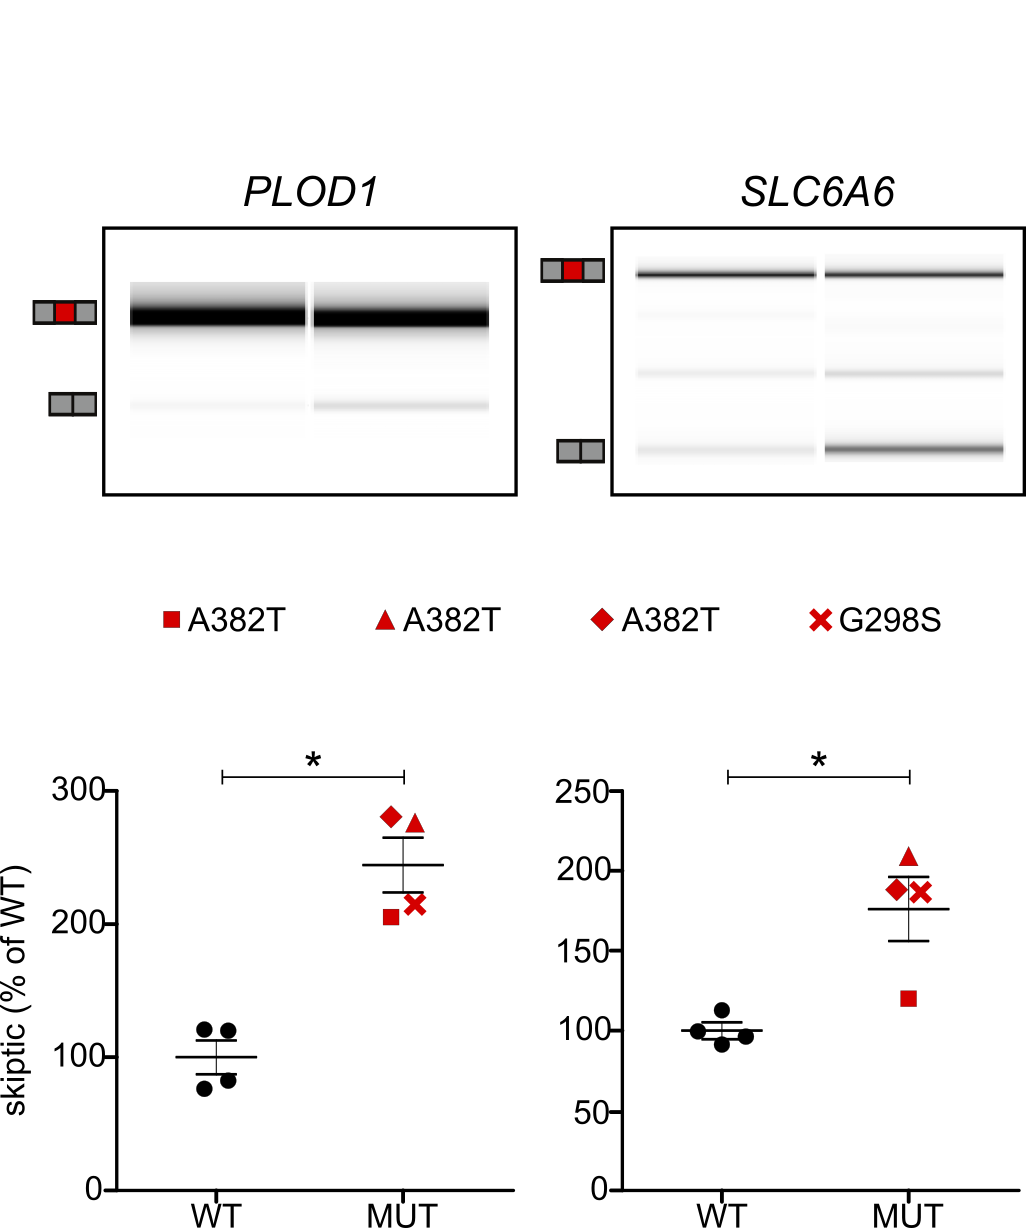
\includegraphics[width=10cm]{Figures/05_tdp_mice/skiptic_patients.png}
	\end{center}
	\label{skiptic_patients}
	\caption{\textbf{Skiptic exon splicing in TARDBP ALS}}
		RT-PCR traces for two skiptic exons in fibroblasts taken from 4 TARDBP ALS patients and 4 non-neurological control lines. For clarity, quantification was taken of the skiptic exon band only instead of the ratio.
\end{figure}



\section{Discussion}

\section{Summary}


% table of all sequencing data used
\begin{table}[h!]
	\caption{List of accessions}
	%\begin{centerline}
	\begin{footnotesize}
		\begin{tabular}{lllll}
		Tissue & Genotype & N &	Read length & Range uniquely mapped reads\\
		\hline	
		Embyonic fibroblasts & RRM2mut &3 &50nt	x 2 & 4-13M\\
			& LCDmut & 3 & 50nt	x	2 & 10-13M\\
			& TDP-43 shRNA & 3 & 50nt x 2 & 7-12M\\
		Embryonic head & RRM2mut & 3 & 40nt	x	2 & 26-48M\\
			& LCDmut & 3 & 40nt	x 2 & 27-34M \\
			%& Double & 3 & 40nt	x 2 & 15-50M \\
		Adult	spinal	cord & RRM2mut & 4 & 75nt x	2 & 41-53M\\
			& LCDmut & 4 & 75nt x 2 & 45-58M\\
		Embryonic	Brain	& RRM2mut & 4 & 100nt x 2 & 31-36M\\
		Adult striatum & TDP-43 ASO & 4 & 75bp x 1 & 35-60M\\
		\citep{Polymenidou2011-hs}
		\end{tabular}
	\end{footnotesize}
%\end{centerline}
\end{table}